\documentclass[12pt,a4paper]{article}
\usepackage[utf8]{inputenc}
\usepackage[spanish]{babel}
\usepackage{amsmath, amssymb, amsfonts}
\usepackage{geometry}
\usepackage{hyperref}
\usepackage{graphicx}
\usepackage{xcolor}
\usepackage{enumitem}
\usepackage{float}

\geometry{left=2.5cm, right=2.5cm, top=2.5cm, bottom=2.5cm}

\title{\textbf{Simulación Bidimensional de un Gas de Esferas Rígidas bajo Compresión Adiabática}}
\author{Reporte Computacional}
\date{\today}

\begin{document}

\maketitle

\section{Fenomenología y Pregunta Física}
El sistema modelado corresponde a un gas ideal bidimensional compuesto por $N$ partículas (discos rígidos) confinadas en una caja rectangular. El sistema experimenta una compresión volumétrica debido a que una de sus paredes laterales (la pared izquierda) actúa como un pistón móvil que avanza con una velocidad constante $v_p$. 

Fenomenológicamente, al no existir intercambio de calor con el exterior, el sistema sufre una \textbf{compresión adiabática}. Cada vez que una partícula colisiona elásticamente con la pared móvil, esta ejerce trabajo sobre la partícula, incrementando su energía cinética y, por ende, la temperatura macroscópica del sistema. Este proceso de compresión está físicamente limitado por el tamaño finito de las partículas, llegando a un punto crítico donde el gas alcanza su empaquetamiento máximo posible.

\textbf{Pregunta física principal:} ¿Cómo evolucionan temporalmente las propiedades termodinámicas macroscópicas (energía interna, temperatura y presión) de un gas de esferas rígidas bidimensional cuando es sometido a una compresión adiabática continua hasta su límite de empaquetamiento crítico?

\section{Modelo Matemático, Variables y Parámetros}
El modelo se construye desde una perspectiva microscópica (cinemática de partículas) para deducir propiedades macroscópicas (termodinámica estadística).

\subsection*{Variables y Parámetros del Sistema}
\begin{itemize}
    \item \textbf{Microscópicos:} Posición $\vec{r}_i = (x_i, y_i)$, velocidad $\vec{v}_i = (v_{xi}, v_{yi})$, masa normalizada $m=1$, radio de interacción $R = \frac{L}{2N}$, y tiempo $t$.
    \item \textbf{Macroscópicos (Caja):} Ancho inicial $L$, altura $h$, área $A(t) = (L - x_{\text{pared}}(t)) \times h$, y velocidad del pistón $v_p$.
    \item \textbf{Constantes:} Constante de Boltzmann normalizada $k_B = 1$. Límite de empaquetamiento hexagonal $\eta = \frac{\pi}{2\sqrt{3}} \approx 0.9069$.
\end{itemize}

\subsection*{Ecuaciones del Modelo}
La energía interna $E$ es puramente cinética. Para $N$ partículas, la energía y la temperatura se relacionan mediante el teorema de equipartición de la energía (en 2D) \cite{schroeder1999thermal}:
$$ E = \sum_{i=1}^{N} \frac{1}{2} m \|\vec{v}_i\|^2 $$
$$ T = \frac{E}{N k_B} $$

La presión $P$ se define en 2D como la fuerza promedio ejercida sobre una longitud. Se calcula a partir de la transferencia de momento lineal ($\Delta p$) de las partículas al colisionar con la pared en un intervalo de tiempo $\Delta t$:
$$ P = \frac{1}{h \Delta t} \sum_{\text{choques}} \Delta p $$
Para la pared móvil, el impulso transferido por una partícula con velocidad $v_x$ es $\Delta p = 2m(v_p - v_x)$.

La simulación se detiene cuando el área disponible se reduce al límite de empaquetamiento hexagonal (con un factor de holgura para evitar divergencias): $A(t) \leq \frac{N \pi R^2}{\eta}$.

\section{Método Computacional y Justificación}

\subsection*{Integración Numérica}
Se utiliza el \textbf{Método de Euler} de primer orden para la actualización espacial en pasos de tiempo discretos $\Delta t$ (\texttt{dt}):
$$ \vec{r}_i(t + \Delta t) = \vec{r}_i(t) + \vec{v}_i(t) \Delta t $$
\textit{Justificación:} Aunque existen integradores más precisos (como Verlet), el método de Euler es suficiente aquí dado que las fuerzas intermoleculares son nulas (potencial de esferas duras). La trayectoria entre colisiones es estrictamente rectilínea y la velocidad es constante.

\subsection*{Resolución de Colisiones}
La detección de colisiones se realiza verificando si la distancia entre centros $\|\vec{r}_i - \vec{r}_j\| \leq 2R$. 
Si existe colisión y las partículas se están acercando (velocidad relativa a lo largo del vector normal $\vec{v}_{\text{rel}} \cdot \vec{N} < 0$), se aplica un impulso instantáneo que conserva el momento lineal y la energía cinética:
$$ J = \frac{-2 (\vec{v}_{\text{rel}} \cdot \vec{N})}{\frac{1}{m_i} + \frac{1}{m_j}} $$
$$ \vec{v}_i' = \vec{v}_i + \frac{J}{m_i} \vec{N}, \quad \vec{v}_j' = \vec{v}_j - \frac{J}{m_j} \vec{N} $$
Para las paredes estacionarias, se invierte especularmente la componente perpendicular de la velocidad. Para la pared móvil, se emplea una transformación de Galileo: $v_x' = 2v_p - v_x$.

\subsection*{Inicialización (Muestreo por Rechazo)}
Para garantizar la estabilidad numérica inicial, las partículas se posicionan utilizando un algoritmo de muestreo por rechazo. Se generan coordenadas aleatorias y se aceptan únicamente si la distancia respecto a las partículas preexistentes supera $2R$, previniendo singularidades energéticas por solapamiento en el $t=0$.

\section{Arquitectura del Programa}
El código está estructurado bajo el paradigma de \textbf{Programación Orientada a Objetos (POO)} en C++, logrando alta modularidad y separación de responsabilidades a través de tres componentes principales:

\begin{enumerate}[label=\textbf{\arabic*.}]
    \item \textbf{Librería Vectorial (\texttt{vector.h} / \texttt{vector.cpp}):}
    Define la clase \texttt{vector2D}. Sobrecarga los operadores matemáticos estándar (\texttt{+}, \texttt{-}, \texttt{*}, \texttt{/}, \texttt{+=}) y funciones amigas para normas euclidianas. Esto permite escribir las ecuaciones del movimiento y de conservación del momento lineal en su forma algebraica natural dentro del código.

    \item \textbf{Clase Partícula (\texttt{collision.h} / \texttt{collision.cpp}):}
    Encapsula el estado físico de la esfera ($r, v, R, m$) y su comportamiento. 
    \begin{itemize}
        \item \texttt{Inicie()}: Método estático que devuelve un \texttt{std::vector<particula>} inicializado sin solapamientos utilizando \texttt{std::mt19937}.
        \item \texttt{coli\_particula()} y \texttt{coli\_pared()}: Implementan la física de detección y respuesta a los choques.
        \item \texttt{generarScriptsGnuplot()}: Rutinas de salida de datos que automatizan la generación de scripts paramétricos para graficar histogramas y animaciones en Gnuplot.
    \end{itemize}

    \item \textbf{Ciclo Principal (\texttt{main.cpp}):}
    Recoge los parámetros iniciales del usuario, invoca el generador de partículas y ejecuta el bucle de integración temporal (\texttt{gen\_frames}). Controla la condición de parada macroscópica (límite de empaquetamiento), gestiona la actualización de la pared móvil, realiza las mediciones estadísticas de $E, T, P$ promediadas temporalmente, y escribe los resultados en archivos \texttt{.dat} para su posterior renderizado.
\end{enumerate}

\section{Experimentos Computacionales}

Para el experimento se emplearon los siguientes parámetros:

\begin{table}[htbp]
    \centering
    \label{tab:parametros-experimento}
    \begin{tabular}{lr}
        \hline
        Parámetro & Valor \\
        \hline
        $n$ & 100 \\
        $R$ & 0.25 \\
        $L\,(\mathrm{m})$ & 50 \\
        $h\,(\mathrm{m})$ & 50 \\
        $v_p\,(\mathrm{m/s})$ & 0.5 \\
        \hline
    \end{tabular}
\end{table}

A continuación se muestra la evolución del sistema en 3 momentos

\begin{figure}[H]
    \centering
    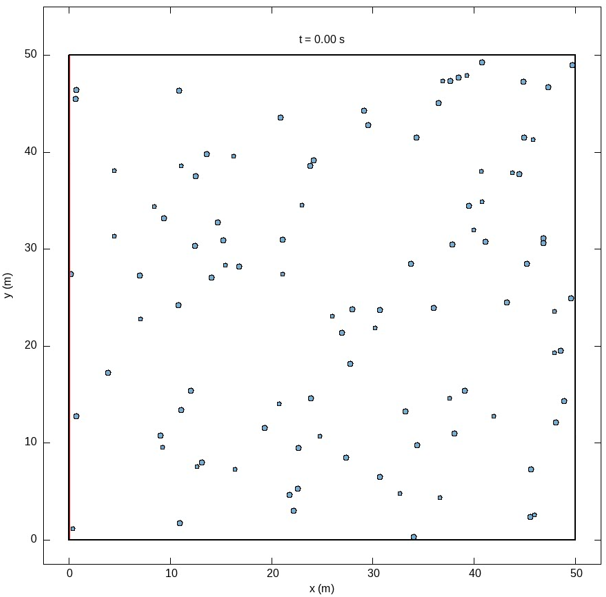
\includegraphics[width=0.32\textwidth]{imagenes/im1.png}\hfill
    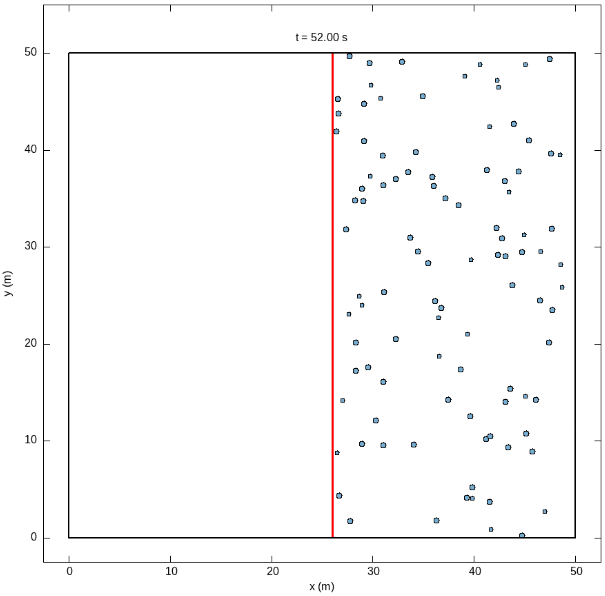
\includegraphics[width=0.32\textwidth]{imagenes/im2.png}\hfill
    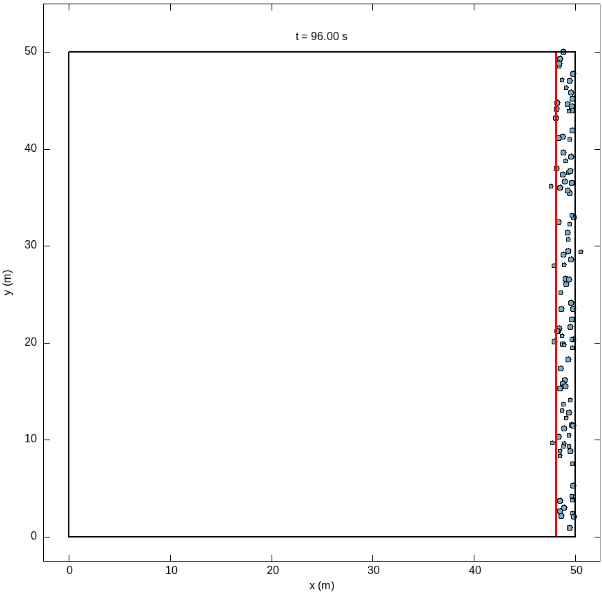
\includegraphics[width=0.32\textwidth]{imagenes/im3.png}
    \caption{Evolución del sistema en tres momentos de la simulación.}
    \label{fig:evolucion-sistema}
\end{figure}

Cerca del límite de empaquetamiento el código empieza a fallar. El aumento en la frecuencia de las colisiones en combinación con la discretización del paso temporal genera que los contactos no se detecten a tiempo; como consecuencia suceden superposiciones entre particulas o entre particula-pared.

Debido a estos fallos es probable que el código no prediga apropiadamente el fenómeno físico cuando el área de la caja se encuentra demasiado cerca del límite de empaquetamiento hexagonal.

\subsection{Evolución de la Energía}

\begin{figure}[H]
    \centering
    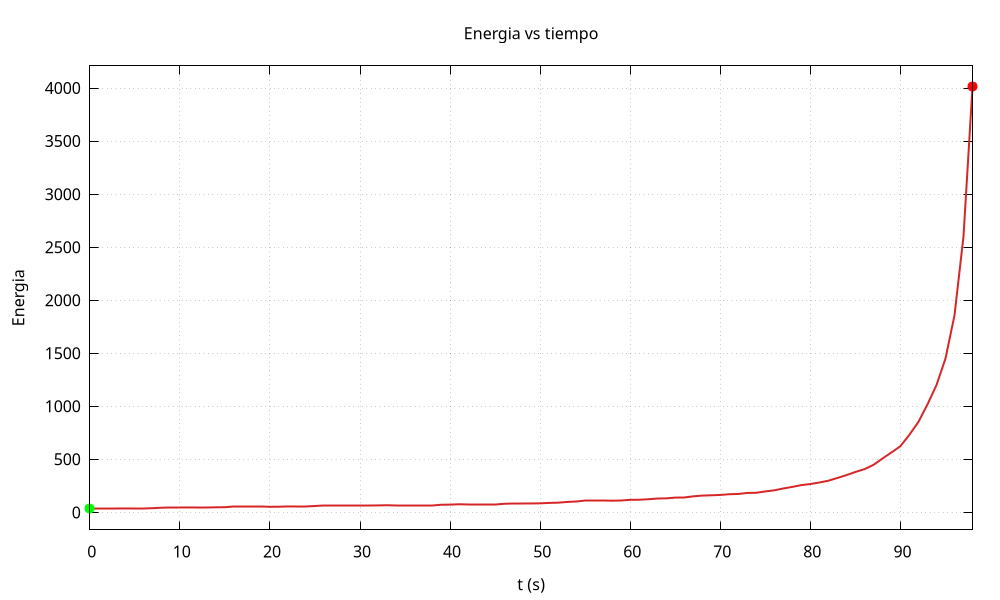
\includegraphics[width=0.8\textwidth]{imagenes/im4.png}
    \caption{Evolución de la energía a lo largo del tiempo}
    \label{fig:example_image}
    
\end{figure}

Dada la ausencia de interacciones potenciales, la energía total del sistema corresponde a la suma de las energías cinéticas de cada partícula. 

El código asigna velocidades aleatorias a cada partícula en el rango $[-1, 1]$ resultando en energías cinéticas bajas.

A medida que el piston avanza y el sistema se comprime, las colisiones entre partículas y con la pared aumentan las velocidades de cada constituyente.

Cerca del límite de empaquetamiento la frecuencia de las colisiones aumenta con creces las velocidades de las partículas, por consecuencia la energía del sistema se dispara.

\subsection{Evolución de la Temperatura}
El código emplea la definición de energía cinética media por partícula para hallar la temperatura, por lo que depende directamente de la energía total del sistema.

\begin{figure}[H]
    \centering
    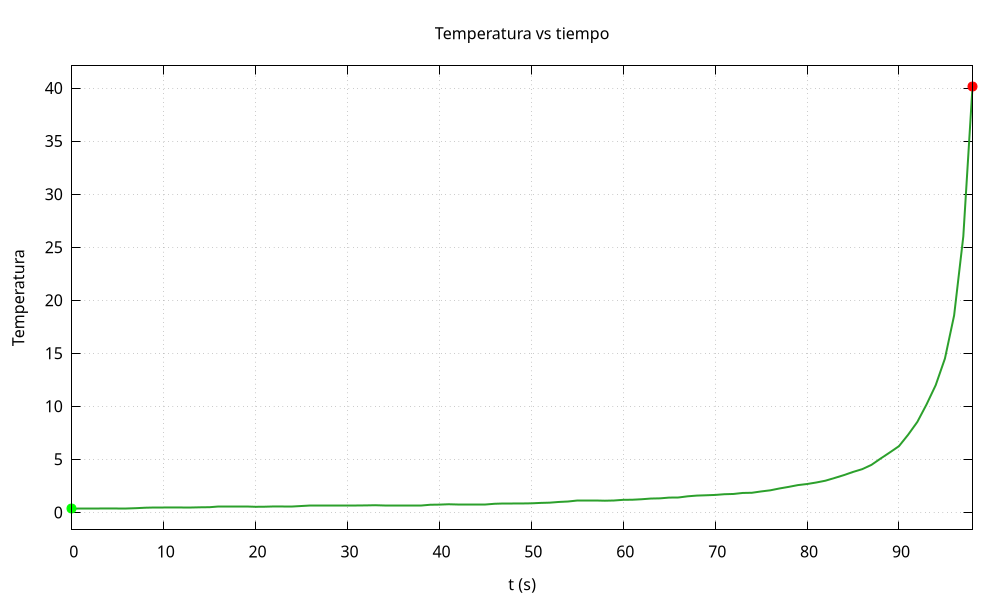
\includegraphics[width=0.8\textwidth]{imagenes/im5.png}
    \caption{Evolución de la temperatura a lo largo del tiempo}
    \label{fig:example_image}
    
\end{figure}

Como es de esperarse la temperatura posee un comportamiento similar a la energía total. Al depender de la energía cinética de las partículas, su valor se dispara cerca del límite de empaquetamiento debido a las frecuentes colisiones entre partículas y con la pared.

Para estos parámetros el sistema alcanza una temperatura cerca de los $40 K$.

\subsection{Evolución de la Presión}

El código calcula la presión a partir del numero de colisiones y el intercambio de momento. Estos cálculos solo se realizaron sobre la pared móvil, que corresponde al fenómeno de interés.

\begin{figure}[H]
    \centering
    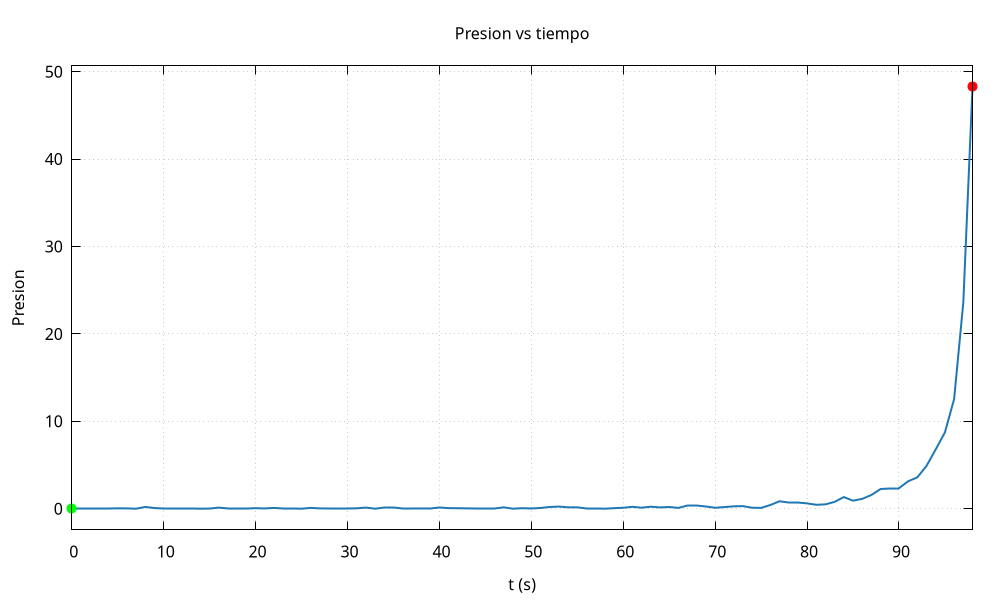
\includegraphics[width=0.8\textwidth]{imagenes/im6.png}
    \caption{Evolución de la presión en la pared móvil a lo largo del tiempo}
    \label{fig:example_image}
\end{figure}

Esta curva cuenta con leves oscilaciones debido a la dependencia del número de colisiones que naturalmente fluctúa durante la evolución del sistema.

A medida que se acerca al límite de empaquetamiento de la caja, la reducción en el espacio libre de las partículas aumenta abruptamente el numero de colisiones con la pared, generando el aumento en la presión.

\section{Conclusiones}

La simulación muestra que la compresión realizada por el pistón incrementa la energía cinética del gas. En consecuencia, la temperatura también aumenta y alcanza aproximadamente $40\,\mathrm{K}$ para los parámetros utilizados. La presión sobre la pared móvil crece conforme disminuye el espacio disponible y aumenta la frecuencia de las colisiones, aunque presenta oscilaciones asociadas a las fluctuaciones en el número de impactos.

Estos resultados describen cualitativamente la respuesta del sistema a la compresión adiabática. Sin embargo, la interpretación de los últimos instantes debe tomarse con cautela: cerca del empaquetamiento, el paso temporal discreto puede impedir la detección oportuna de algunos choques y producir superposiciones. Por tanto, las predicciones en esa región son menos fiables; reducir el paso temporal o emplear un método de detección de colisiones más preciso permitiría mejorar el análisis cerca del límite.

\renewcommand{\refname}{Referencias}
\bibliographystyle{plain}
\bibliography{referencias}

\end{document}
